\chapter{Reference}

\section{Operations}\label{Operations}

\subsection{Special
  constants}\label{Operation:euler}\label{Operation:pi}\label{Operation:zero}\label{Operation:one}
\label{Operation:inf}

Some special constants ($e=2.72\ldots$, $\pi=3.14\ldots$, 0, 1,
$\infty$).

\subsection{Percent} \label{Operation:percent} Multiplies input by
100.

\subsection{add +}\label{Operation:add} Add multiple numbers together. The input
ports allow multiple wires, which are all summed. If an input port is
unwired, it is equivalent to setting it to zero.

\subsection{subtract $-$}\label{Operation:subtract} Subtract two numbers. The input
ports allow multiple wires, which are summed prior to the subtraction
being carried out. If an input port is unwired, it is equivalent to
setting it to zero. Note the small `+' and `$-$' signs on the input
ports indicating which terms are added or subtracted from the result.

\subsection{multiply $\times$}\label{Operation:multiply} Multiply numbers with each
other. The input ports allow multiple wires, which are all multiplied
together. If an input port is unwired, it is equivalent to setting it
to one.

\subsection{divide $\div$}\label{Operation:divide} Divide a number by another. The
input ports allow multiple wires, which are multiplied together prior
to the division being carried out. If an input port is unwired, it is
equivalent to setting it to one. Note the small `$\times$' and
`$\div$' signs indicating which port refers to the numerator and which
the denominator.

\subsection{log}\label{Operation:log} Take the logarithm of the $x$ input port, to
base $b$. The base $b$ needs to be specified --- if the natural
logarithm is desired ($b=e$), use the \htmlref{ln
  operator}{Operation:ln} instead.

\subsection{pow $x^y$}\label{Operation:pow} Raise one number to the power of another. The
ports are labelled $x$ and $y$, referring the the formula $x^y$.

\subsection{lt $<$}\label{Operation:lt} Returns 0 or 1, depending
on whether $x<y$ is true (1) or false (0).

\subsection{le $\le$}\label{Operation:le} Returns 0 or 1, depending
on whether $x\le y$ is true (1) or false (0).

\subsection{eq $=$}\label{Operation:eq} Returns 0 or 1, depending
on whether $x=y$ is true (1) or false (0).

\subsection{min}\label{Operation:min} Returns the minimum of $x$ and
$y$.

\subsection{max}\label{Operation:max} Returns the maximum of $x$ and
$y$.

\subsection{and $\wedge$}\label{Operation:and_} Logical and of $x$ and $y$, where
$x\le 0.5$ means false, and $x>0.5$ means true. The output is 1 or 0,
depending on the result being true (1) or false (0) respectively.

\subsection{or $\vee$}\label{Operation:or_} Logical or of $x$ and $y$, where $x\le0.5$
means false, and $x>0.5$ means true. The output is 1 or 0, depending
on the result being true (1) or false (0) respectively.

\subsection{not $\neg$}\label{Operation:not_} The output is 1 or 0, depending
on whether $x\le0.5$ is true (1) or false (0) respectively.

\subsection{time $t$}\label{Operation:time}  Returns the current value
of system time.

\subsection{Gamma $\Gamma$}\label{Operation:Gamma} Returns the Gamma
function of its argument:
\begin{displaymath}
  \Gamma(x)=\int_0^\infty t^{x-1}e^{-t}dt
\end{displaymath}

\subsection{Factorial !}\label{Operation:fact} Returns the factorial
of its argument:
\begin{eqnarray*}
  0!&=&1\\
  n! &=& \prod_{i=1}^n i\\
\end{eqnarray*}
Note:
\begin{displaymath}
  n!=\Gamma(n+1)
\end{displaymath}
which is how it is implemented in Minsky.

\subsection{Polygamma $\psi^{(n)}(x)$}\label{Operation:polygamma} Returns the polygamma function
of the first argument $x$, with the order $n$ being given by the floor
of the second argument.
\begin{displaymath}
  \psi^{(n)}(x)=\frac{d^{n+1}}{dx^{n+1}}\ln\Gamma(x)
\end{displaymath}

It relationship to the derivative of the Gamma function (and
factorials) is why Minsky provides this function.

\subsection{differentiate $d/dt$}\label{Operation:differentiate}
Symbolically differentiates its input with respect to system time,
producing d/dt[input].  For further explanation regarding
differentiation, see
\href{https://en.wikipedia.org/wiki/Derivative}{this wikipedia page}.

% \subsection{data }\label{Operation:data} \buttonIcon{data.eps} A
% data interpolation widget. The data can be imported from a file
% containing two values on each line, eg:
% \begin{quote}
%   \begin{tabular}{rr}
%0.1 &0.3\\
%0.5 &0.7\\
%0.9 &1\\
%\end{tabular}
% \end{quote}
%
% If the input is less than the minimum key value (0.1 here), then the
% operation outputs the corresponding value (0.3). Similarly if the
% input is greater than the maximum (0.9), the corresponding value (1)
% is output. If it lies in between two keys (eg 0.2), the the output
% is linearly interpolated (0.4).
%
% Alternatively, the data block can be initialised by a random number
% generator, which is a way of introducing random numbers\index{random
% numbers} into the simulation. The parameters, the minimum and
% maximum values of the function's domain, and the number of random
% samples over that domain, are all required.
%
% \begin{center}
%   \begin{tabular}{cc}
%  \resizebox{5.17cm}{!}{\includegraphics{images/initRandom.eps}} &
%  \resizebox{0.5\textwidth}{!}{\includegraphics{images/randomExample.eps}}
%  \end{tabular}
%\end{center}
%
%More formally, a data block is an empirical function, based on a
% table of pairs of values ($x_i, y_i, i=1\ldots n, x_{i+1}>x_i$) read
% in from a file. The function's output is linearly interpolated from
% the data, ie:
% \begin{displaymath}
%f(x) = \left\{
%\begin{array}{cl}
%y_1 & x < x_1\\
%y_n & x\geq x_n\\
%\frac{y_i(x_{i+1}-x)+y_{i+1}(x-x_i)}{x_{i+1}-x_i} & x_i \leq x <
%x_{i+1}\\
%\end{array}
%\right.
%\end{displaymath}

\subsection{User defined
  function}\label{Operation:userFunction}\label{UserFunction}

A user defined function is a functioned defined by an algebraic
expression. Support for this feature is courtesy of the wonderful
\htmladdnormallink{exprtk}{http://www.partow.net/programming/exprtk/index.html}
library developed by Arash Partow.

A user defined function has a {\em name}, {\em parameters} and an {\em
  expression}. Example expressions are things like \verb'x+y' or
\verb'sin(x)'. More details of the sorts of expressions possible can
be found in the \htmlref{User Defined Functions}{ExprTk} section of
the manual.

The parameters are specified as part of the name, so a user defined
function adding x and y would be called \verb'useradd(a,y)' and the
sin example might be called \verb'mysin(x)'. Functions with up to two
arguments can be wired on the canvas. User defined functions can call
other user defined functions, so specifiying more than 2 parameters
can be a useful thing to do.

\subsection{copy}\label{Operation:copy} This just copies its input to its output,
which is redundant on wiring diagrams, but is needed for internal
purposes.

\subsection{integrate $\int dt$}\label{IntOp}  Creates an integration (or stock)
variable. Editable attributes include the variable's name and its
initial value at $t=0$. The function to be integrated needs to be
connected to the top port, labelled `$f$'. The bottom port, labelled `0', can optionally be connected
to a constant, parameter or variable, which is used to specify the
initial value of the integral.

Note that the units of the integral operator are given by the units of
the input, multiplied by the \htmlref{time unit}{RungeKutta}, but the units of the {\em integral's
  variable} are user specified. It is an error for these to be
mismatched, and running {\em dimensional analysis} from the
\htmlref{File menu}{File} will check for the
  consistency of this. Note that the user specified units in the
  integral variable can be used to dimension up the integral if the
  integral variable is connected to the integral's input.

\subsection{sqrt $\surd$}\label{Operation:sqrt} This produces the square root of 
the input value. For example, connecting the value of 9 with the
``sqrt'' block will produce the value of 3.

\subsection{exp}\label{Operation:exp} Connecting a variable (for example, ``time'')
to this block will produce the exponential function $e^{x}$ where x is
the input variable.

\subsection{ln}\label{Operation:ln} Produces a natural logarithm of the input, to the base of e.
This takes the equation $\log_{e} x$ where $x$ is the input.

\subsection{sin}\label{Operation:sin} Produces a sine function of the input. For example, 
connecting a ``time'' block to this function, and then to a graph,
will produce a sine wave.  For further explanation regarding
trigonemtric functions, see \htmladdnormallinkfoot{this wikipedia
  page}{https://en.wikipedia.org/wiki/Trigonometric\_functions}.

\subsection{cos}\label{Operation:cos} Produces a cosine function of the input. For example, 
connecting a ``time'' block to this function, and then to a graph,
will produce a cosine wave.  For further explanation regarding
trigonemtric functions, see \htmladdnormallinkfoot{this wikipedia
  page}{https://en.wikipedia.org/wiki/Trigonometric\_functions}.

\subsection{tan}\label{Operation:tan} Produces a tangent function of the input. For example, 
connecting a ``time'' block to this function, and then to a graph,
will produce a tangent graph.  For further explanation regarding
trigonemtric functions, see \htmladdnormallinkfoot{this wikipedia
  page}{https://en.wikipedia.org/wiki/Trigonometric\_functions}.

\subsection{asin}\label{Operation:asin} Produces an arc sine function of the input, 
or the inverse of the sine function. For further explanation regarding
trigonemtric functions, see \htmladdnormallinkfoot{this wikipedia
  page}{https://en.wikipedia.org/wiki/Trigonometric\_functions}.

\subsection{acos}\label{Operation:acos} Produces an arc cosine function of the input, 
or the inverse of the cosine function. For further explanation
regarding trigonemtric functions, see \htmladdnormallinkfoot{this
  wikipedia
  page}{https://en.wikipedia.org/wiki/Trigonometric\_functions}.

\subsection{atan}\label{Operation:atan} Produces an arc tangent function of the input, 
or the inverse of the tangent function. For further explanation
regarding trigonemtric functions, see \htmladdnormallinkfoot{this
  wikipedia
  page}{https://en.wikipedia.org/wiki/Trigonometric\_functions}.

\subsection{sinh}\label{Operation:sinh} hyperbolic sine function
$\frac{e^x-e^{-x}}2$
\subsection{cosh}\label{Operation:cosh} hyperbolic cosine function
$\frac{e^x+e^{-x}}2$
\subsection{tanh}\label{Operation:tanh} hyperbolic tangent function
$\frac{e^x-e^{-x}}{e^x+e^{-x}}$
\subsection{abs $|x|$}\label{Operation:abs} absolute value function
\subsection{floor $\lfloor x\rfloor$}\label{Operation:floor} The
greatest integer less than or equal to $x$.
\subsection{frac}\label{Operation:frac} Fractional part of $x$, ie
$x-\lfloor x\rfloor$.

\section{Tensor operations}\label{tensor
  operations}\index{tensor|operations}

In the following operations, an axis argument can be supplied in the
operation edit dialog. The axis name is symbolic and available in a
drop down box. If the axis name is not specified, then the operation
will be applied as though the input was flattened (unrolled to a
vector), and then the result reshaped to the original tensor.

\subsection{sum $\sum$}\label{Operation:sum} Sum along a given
axis.

\subsection{product $\prod$}\label{Operation:product} Multiply along a
given axis.

\subsection{infimum}\label{Operation:infimum} Return the least value
along a given axis.

\subsection{supremum}\label{Operation:supremum} Return the greatest value
along a given axis.

\subsection{any}\label{Operation:any} Return 1 if any value
along a given axis is nonzero, otherwise return 0 if all are zero.

\subsection{all}\label{Operation:all} Return 1 if all values
along a given axis are nonzero, otherwise return 0 if any are zero.

\subsection{infindex}\label{Operation:infIndex} Return the index of
the least value along a given axis.

\subsection{supindex}\label{Operation:supIndex} Return the index of
the greatest value along a given axis.

\subsection{running sum $\sum+$}\label{Operation:runningSum} Computes
the running sum of the input tensor along a given axis. For example,
take this rank 2 tensor:

\begin{displaymath}
  \left(
    \begin{array}{cccc}
      1& 2& 3& 4 \\
      5& 4& 3& 2 \\
      8& 7& 6& 5
    \end{array}
  \right)
\end{displaymath}

The running sum of this tensor, along the horizontal dimension, is:

\begin{displaymath}
  \left(
    \begin{array}{cccc}
      1& 3& 6& 10 \\
      5& 9& 12& 14 \\
      8& 15& 21& 26
    \end{array}
  \right)
\end{displaymath}

\subsection{running product $\prod+$}
\label{Operation:runningProduct} Computes the running product of the
input tensor along a given axis. For example, take this rank 2 tensor:

\begin{displaymath}
  \left(
    \begin{array}{cccc}
      1& 2& 3& 4\\ 
      5& 4& 3& 2\\ 
      8& 7& 6& 5 
    \end{array}
  \right)
\end{displaymath}

The running product of this tensor, along the horizontal dimension,
is:

\begin{displaymath}
  \left(
    \begin{array}{cccc}
      1& 2& 6& 24\\ 
      5& 20& 60& 120\\ 
      8& 56& 336& 1680 
    \end{array}
  \right)
\end{displaymath}

\subsection{difference $\Delta^-,\Delta^+$}\label{Operation:difference}\label{Operation:differencePlus}
Computes the nearest neighbour difference along a given direction. The
optional argument ($\delta$) can be used to specify the number of
neighbours to skip in computing the differences. The length of the
dimension being differenced is reduced by $\delta$ in the result.

It comes in two different forms which differ only in how the resultant
x-vector is calculated. $\Delta^-_i=x_i-x_{i-\delta}$, and
$\Delta^+_i=x_{i+\delta}-x_i$, where $i$ refers to the x-vector index.

\subsection{index}\label{Operation:index}

Returns the index within the hypecube where the input is true (ie
$>0.5$). For example, where
\begin{eqnarray*}
  \iota(3,3) &=& \left(\begin{array}{ccc}
                         0 & 3 & 6 \\
                         1 & 4 & 7 \\
                         2 & 5 & 8 \\
                       \end{array}\right),\\
  \mathrm{idx}(\iota(3,3)<5) &=&
                                 \left(\begin{array}{ccc}
                                         0 & 3 &\\
                                         1 & 4 &\\
                                         2 & &
                                       \end{array}\right),\\
\end{eqnarray*}
Note that the output array has the same shape as the input, with
unused values padded with NANs (missing value).

Dimension and argument parameters are unused.


\subsection{gather}\label{Operation:gather}

Gather collects the values at index locations indexed by the second
argument. The output tensor has shape
$[i_0, \ldots i_{ir}, a_0,\ldots a_{j-1},a_{j+1},\ldots a_{ar}]$ where
$[a_0,\ldots,a_{ar}]$ is the shape of the first argument, and
$[i_0,\ldots,i_{ir}]$ is the shape of the second second (index)
argument, and $j$ is the axis along which the gather is performed.

If the index is not an integer, the gather will linearly interpolate
between the values on either side. So, for example,
$x[2.5] = 0.5 (x[2]+x[3])$.

If the index value is outside the range of the
\htmlref{x-vector}{x-vector} along the axis being gathered, then NAN is assigned
to that tensor element.

\subsection{inner product $\cdot$}\label{Operation:innerProduct}
Computes
\begin{displaymath}
  z_{i_1,\ldots,i_{r_x-1},j_1,\ldots,j_{r_y-1}} =
  \sum_k x_{i_1\ldots,i_{a-1},k,i_{a+1}\ldots,i_{r_x-1}}
  y_{j_1,\ldots,j_{r_y-1},k},
\end{displaymath}
where $a$ is the given axis, and $r_x$ and $r_y$ are the ranks of $x$
and $y$ respectively.

\subsection{outer product $\otimes$}\label{Operation:outerProduct}
Computes
\begin{displaymath}
  z_{i_1,i_2,\ldots,i_{r_x},j_1,\ldots,j_{r_y}} =
  x_{i_1,,i_2,\ldots,i_{r_x}}y_{j_1,\ldots,j_{r_y}}.
\end{displaymath}
where $r_x$ and $r_y$ are the ranks of $x$ and $y$ respectively.

\subsection{Meld}\label{Operation:meld}

The meld operation merges the hypercubes of its input tensors. The
value at a given hypercube value is given by the value of the first
tensor that has a value defined at that hypercube point. So ordering of
input tensors does matter where the data is inconsistent between input
tensors.

For example, consider the following inputs and x-vectors:

\begin{enumerate}
\item \label{ex1} $\{1.0, 2.0, 3.0\}$ with x-vector $\{1,2,3\}$, and
  \item \label {ex2} $\{0.0,1.5,4.0\}$ with x-vector $\{0,2,4\}$
  \end{enumerate}
then the resultant output has x-vector $\{0,1,2,3,4\}$ and the values
are $\{0.0,1.0,2.0,3.0,4.0\}$ if \ref{ex1} is connected to port 1 and
\ref{ex2} connected to port 2. If they were connected the other way
around, the the values would be $\{0.0,1.0,1.5,3.0,4.0\}$.

\subsection{Merge}\label{Operation:merge}

The merge operation takes $n$ tensors, finds the union hypercube (ie
the hypercube that contains all the input tensor hypercubes) and
spreads the tensors as necessary to make them conformant. Finally,
the resultant tensor has an additional string dimensioned axis, each
element of which is one of the input tensors. This dimension should be
named using the operation edit dialog. It is an error for a hypercube
to contain more than one axis with the same name.

\subsection{Slice}\label{Operation:slice}

Slice will cut off a tensor along a given axis by the argument, as
configured in the operation edit dialog. For
example $\mathrm{slice}(\{x_1,x_2,\ldots x_n\},
  3)=\{x_1,x_2,x_3\}$. If the tensor is rank one (ie a vector), it is
  not necessary to specify the axis.

If the slice argument is negative, then it refers to the number of
elements from the end of that axis. For example $\mathrm{slice}(\{x_1,x_2,\ldots x_n\},
  -3)=\{x_{n-3},x_{n-2},x_{n-1}\}$.

\subsection{Size}\label{Operation:size}

Size refers to the number of elements along a named dimension given by
the operation axisargument - eg a $3\times2$ rank 2 tensor with named
axes ``0'' and ``1'', size(``1'')==2.

If the axis argument is left blank, the size returns the total number
of elements present in the tensor. This may be less than the product
of axis sizes if the data is sparse.

\subsection{Shape}\label{Operation:shape}

Returns a vector of axis sizes. Coupling this operation with a
\htmlref{gather}{Operation:gather} operation
and variable would allow you interactively select axis size.

\subsection{Mean}\label{Operation:mean}

Returns the mean (or average) along a named dimension of all
elements present. If the dimension is not named, then the mean is
over all elements present in the tensor. Note that missing elements
are not counted.

\subsection{Median}\label{Operation:median}

Returns the median  along a named dimension of all
elements present. If the dimension is not named, then the median is
over all elements present in the tensor. 

\subsection{Standard Deviation}\label{Operation:stdDev}

Returns the standard deviation along a named dimension of all
elements present. If the dimension is not named, then the standard
deviation is over all elements present in the tensor. Note that
missing elements are not counted.

\begin{displaymath}
  \sigma = \frac1{N-1}\sum_i^N (x_i-\langle x\rangle)^2
\end{displaymath}

\subsection{$k$-th moment}\label{Operation:moment}
  
Returns the $k$-th moment about the mean along a named dimension of
all elements present. $k$ is specified by the numerical argument of
the operation, which defaults to 1 (hence the result will be 0 in that
case). If the dimension is not named, then the $k$-th moment is over
all elements present in the tensor. Note that missing elements are not
counted.

\begin{displaymath}
  \langle\Delta x^k\rangle = \frac1N\sum_i(x_i-\langle x\rangle)^k
\end{displaymath}

Also
\begin{displaymath}
  \sigma^2 = \frac{N}{N-1}\langle\Delta x^2\rangle
\end{displaymath}


\subsection{Histogram}\label{Operation:histogram}

Computes the histogram along a named dimension of all
elements present. If the dimension is not named, then the histogram
is over all elements present in the tensor. The number of bins is
specified by the numeric argument to the operation.

\begin{center}
  \resizebox{\textwidth}{!}{\includegraphics{images/histogram.eps}}

  {\em An example usage of the histogram operation}
\end{center}

\subsection{Covariance}\label{Operation:covariance}

Computes the covariance of two tensors along named dimension. If the
inputs are of rank $N$ and $M$ respectively, the output will be a
$(N-1)\times(M-1)$ rank tensor, where the $(i,j)$ element is the
covariance of the $i$-th slice of the first argument along the named
dimension, and the $j$-th slice along the named dimension. As such, it
is conformant with the definition of {\tt cov} function in Octave, but
not with the equivalently named function in Matlab:
\begin{quote}
     Compatibility Note:: Octave always treats rows of X and Y as
     multivariate random variables.  For two inputs, however, MATLAB
     treats X and Y as two univariate distributions regardless of their
     shapes, and will calculate ‘cov ([X(:), Y(:)])’ whenever the number
     of elements in X and Y are equal.  This will result in a 2x2
     matrix.  Code relying on MATLAB’s definition will need to be
     changed when running in Octave.
   \end{quote}

If only a single argument $x$ is supplied to the covariance, then the
result is equivalent to cov$(x,x)$, ie each slice is covaried with
each other slice.
   
   The formula for covariance between stochastic variables $x$ and $y$
   is
   \begin{displaymath}
     \mathrm{cov}(x,y)=\frac1{N-1}\sum_i(x_i-\langle
     x\rangle)(y_i-\langle y\rangle)
   \end{displaymath}

   \subsection{Correlation coefficient $\rho$}\label{Operation:rho}

   See
   \htmlref{covariance}{Operation:covariance}
   for the interpretation of tensor valued arguments. The correlation
   coefficient is defined as

   \begin{displaymath}
     \rho(x,y)=\frac{\mathrm{cov(x,y)}}{\sigma(x)\sigma(y)}
   \end{displaymath}
   

\section{Switch}\label{SwitchIcon}

\buttonIcon{switchIcon.eps} A switch block (also known as a case
block, or select in the Fortran world) is a way of selecting from a
range of alternatives according to the value of the input, effectively
defining a piecewise function.

\begin{center}
  \resizebox{\textwidth}{!}{
\includegraphics{images/switch.eps}} {\em
    An example switch block with 3 cases}
\end{center}

The default switch has two cases, and can be used to implement an
if/then/else construct. However, because the two cases are 0 and 1, or
false and true, a two case switch statement will naturally appear
``upside down'' to how you might think of an if statement. In other
words, it looks like:

\parbox{\textwidth}{
  {\tt if not }{\em condition} {\tt then}\\
  \ldots
  {\tt else}\\
  \ldots }

You can add or remove cases through the context menu.

\section{Variables}\label{Variables}\label{Variable:constant}\label{VarConstant}\label{Variable:parameter}
\label{Variable:flow}\label{Variable:integral}\label{Variable:stock}

Variables represent values in a calculation, and come in a number of
varieties:
\begin{description}
\item[Constants] represent an explicit numerical value, and do not
  have a name. Their graphical representation shows the actual value
  of the constant.
\item[Parameters] are named constants. All instances of a given name
  represent the same value, as with all other named variables, so
  changing the value of one parameter, either through its edit menu,
  or through a slider, will affect all the others of that
  name. Parameters may be \htmlref{imported from a CSV file}{CSV
    import}, which is one way of inserting a tensor into the
  simulation.
\item[Flow variables] have an input port that defines how the value is
  to be calculated. Only one flow variable of a given name can have
  its input port connected, as they all refer to the same quantity. If
  no input ports are connected, then flow variables act just like
  parameters.
\item[Integral variables] represent the result of integrating its
  input over time by means of the differential equation solver. The
  integrand is represented by the input to an integral operator that
  is attached to the integral variable.
\item[Stock variables] are the columns of Godley tables, and represent
  the integral over time of the sum of the flow variables making up
  the column.
\end{description}

Variables may be converted between types in the variable edit menu,
available from the context menu, subject to certain rules. For
example, a variable whose input is wired anywhere on the canvas cannot
be changed from ``flow''. Stock variables need to be defined in a
Godley table, and so on.

\subsection{Variable names}

Variable names uniquely identify variables. Multiple icons on the
canvas may have the same name --- they all refer to the same
variable. Variable names have scope, which is either local (no initial
`:'), belonging to an outer \htmlref{group}{Group} (indicated by a
leading `:' on the inner group variable, and the outer group variable
having no such leading `:'), or completely global otherwise. You may
select a variable name from a drop down list in the ``name'' combo
box, which makes for an easier way of selecting exactly which variable
you want.

\subsection{Initial conditions}\label{var:init}\index{initial
  conditions}

Variable initial conditions can be defined through the ``init value''
field of the variable edit menu, or in the case of Godley table stock
variables, through the initial condition row of the Godley table. An
initial value can be a simple number, or it can be a multiple of
another named variable (or parameter). In case of symbolic
definitions, it would be possible to set up a circular reference where
the initial value of variable A is defined in terms of the initial
value of variable B, which in turn depends on the intial value of
A. Such a pathological situation is detected when the system is reset.

\subsection{Tensor valued initial
  conditions}\label{tensor-init}\index{initial conditions|tensor}

There is also a simple functional language, which allows for the
generation of tensor-valued operations. These functions take the form
{\em func}$(n_1,n_2,\ldots,n_r)$ where $r$ is the desired rank, and
$n_1,n_2,$ etc are the dimensions of the tensor. Available functions
include:

\begin{tabular}{|r|l|}
  \hline
  name & description\\\hline
  \verb+one+ & the tensor is filled with `1'\\
  \verb+zero+ & the tensor is filled with `0'\\
  \verb+iota+ & the arithmetic sequence $(0,1,...\prod_in_i)$\\
  \verb+eye+ & diagonal elements filled with `1', offdiagonal `0'\\
  \verb+rand+ & tensor filled with random numbers in the range $[0,1)$\\
  \hline
\end{tabular}
\index{one}\index{zero}\index{iota}\index{eye}\index{rand}

\begin{itemize}
\item \verb+eye+ is equivalent to \verb+one+ for vectors.
\item \verb+rand+ generates different random numbers each time the
  simulation is reset, and uses the clib \verb+rand()+ function.
\end{itemize}


\subsection{Sliders}

From the context menu, one can select a slider to be attached to a
variable, which is a GUI ``knob'' allowing one to control a variable's
initial value, or the value of a parameter or constant. Adjusting the
slider of an integral (or stock) variable while the system is running
actually adjusts the present value of the variable. The sliders can
also be adjusted using the keyboard arrow keys.

Slider parameters are specified in the edit menu: max, min and step
size. A relative slider means that the step size is expressed as a
fraction of max-min.

\subsection{Importing a parameter from a CSV file}\label{CSV import}
\index{CSV|import}\label{Operation:csvImport}

After creating a parameter from the ``Variable'' drop-down in the
``Insert'' menu, right-clicking the parameter and selecting the option
to ``Import CSV'', will open a dialogue box that allows you to select
a CSV file. Upon selecting the file, a dialog is opened, allowing you
to specify assorted encoding parameters.

An alternative is to click on the ImportData icon
\buttonIcon{importData.eps}, which will create a new parameter for you
to import the data into.

The dialog looks somewhat like this:

\begin{center}
  \resizebox{\textwidth}{!}{\includegraphics{images/CSVimportDialog.eps}}
\end{center}

Quick instructions:
\begin{itemize}
\item Data is typically rightmost columns. Click to set the top left
  cell of the data. Columns to the left will be marked as axes.
\item Select ``axis'' in the Dimension dropdown to include a column as
  an axis. Column data turns blue.
\item Select ``ignore'' in the Dimension dropdown to exclude a
  column. Column data turns red.
\item Select ``data'' in the Dimension dropdown to treat a column as a
  data column. Column data turns black.
\item Select Type for included axis columns. Select one of three
  types:
  \begin{description}
  \item[string] most general type, data treated as is.
  \item[value] value data must be numerical and not quoted, e.g. 1, 2
  \item[time] data must refer to date-time data. Format field may be
    used to control interpretation of this data. Blank format assumes
    data contains year/month/day/hour/minute/second separated by some
    non-numerical character. If fewer than 6 numerical fields present,
    smallest units are set to minimum value (0 or 1 respectively).
  \end{description}
\item Click OK button.
\item Data is imported into the parameter.
\item You may now need to set units for the imported data field, which
  is located at Edit $\rightarrow$ Dimensions.
\end{itemize}

In the case shown above, the system has automatically guessed that the
data is 3 dimensional, and that the first 3 columns give the axis
labels for each dimension (shown in blue), and the 4th column contains
the data. The first row has been automatically determined to be the
first row of the file --- with the dimension names are shown in green.

In this case, the automatic parsing system has worked things out
correctly, but often times it needs help from the computer user. An
example is as follows:

\begin{center}
  \resizebox{\textwidth}{!}{\includegraphics{images/CSVimportDialogFail.eps}}
\end{center}

In this example, Minsky has failed to determine where the data starts,
probably because of the columns to the right of the ``Price''
columns. So the first thing to do is tell it where the data is located
by clicking on the first cell of the data region.

\begin{center}
  \resizebox{\textwidth}{!}{\includegraphics{images/CSVimportDialogSelectData.eps}}
\end{center}

Note that this causes all columns to the right of ``Price paid'' to be
treated as data, which is not right since the columns to the right of
``Propieter'' are text based columns, not data. So we need to mark
those columns as either ``axis'' or ``ignore''. To do that, select
drag on the header field, which will cause those columns to be
selected, like so:

\begin{center}
  \resizebox{\textwidth}{!}{\includegraphics{images/CSVimportDialogSelectedColumns.eps}}
\end{center}

Then in the dimensions row, select ``axis'', which flips the selected
columns:

\begin{center}
  \resizebox{\textwidth}{!}{\includegraphics{images/CSVimportDialogSelectedAxes.eps}}
\end{center}



Now the axes index labels are rendered in blue, the axes names in
green and the data is in black. In this example, some axes have unique
values, which are not particularly useful to scan over. Other examples
might have columns that duplicate others, in effect the data is a
planar slice through the hypercube. We can remove these axes from the
data by marking the column ``ignore'' in the ``Dimension'' row. The
deselected columns are rendered in red, indicating data that is
commented out:

\begin{center}
  \resizebox{\textwidth}{!}{\includegraphics{images/CSVimportDialogAxesDeselected.eps}}
\end{center}

In this example, the axis names has not been correctly
inferred. Whilst, one can manually edit the axis names in the ``Name''
line, a quick shortcut is to drag ``Header'' and drop it on
``Name''. (Note the intention is for this to be the case - currently
each column name has to be set individually).

\begin{center}
  \resizebox{\textwidth}{!}{\includegraphics{images/CSVimportDialogAxesNamed.eps}}
\end{center}


The Date column is current parsed as strings, which not only will be
sorted incorrectly, but even if the data were in a YYYYMMDD format
which is sorted correctly, will not have a uniform temporal
spacing. It is therefore important to parse the Date column as
temporal data, which is achieved by changing the column type to
``time'', and specifying a format string, which follows strftime
conventions with the addition of a quarter specifier (\verb+%Q+).
\index{strftime format specifier}\label{strftime format specifier}

If your temporal data is in the form Y*M*D*H*M*S, where * signifies
any sequence of non-digit characters, and the year, month, day, hour
minutes, second fields are regular integers in that order, then it
suffices to use the blank format string \index{blank strftime
  format}. If some of the fields are missing, eg minutes and seconds,
then they will be filled in with sensible defaults.

\begin{center}
  \resizebox{\textwidth}{!}{\includegraphics{images/CSVimportDialogTimeFormat.eps}}
\end{center}

\begin{table}
  \begin{tabular}{|c|l|}
    \hline Code & Description \\\hline
    \%a or \%A &  The name of the day of the week according to the current locale,
                 in abbreviated form or the full name.\\
    \%b or \%B &  The month name according to the current locale,  in  abbreviated
                 form or the full name.\\
    \%d & Day of month in range 01 to 31\\
    \%H & Hour in range 0 to 23\\
    \%I & Hour in range 1 to 12\\
    \%m & Month as a decimal number (01 to 12)\\
    \%M & Minute in range 00 to 59\\
    \%Q & Quarter (0=1st January, 1=1st March etc)\\
    \%p & AM or PM\\
    \%s & Number of seconds since epoch (1st January 1970)\\
    \%S & Seconds in range 00 to 59 \\
    \%y & Two digit year YY\\
    \%Y & Four digit year YYYY\\
    \%z & numerical timezone offset\\
    \%Z & Timezone name\\
    \%\% & Literal \% character\\
    \hline
  \end{tabular}
  \caption{Table of strftime codes}
  \label{Strftime code}
\end{table}

Strftime formatted string consists of escape codes (with leading \%
characters). All other characters are treated as matching literally
the characters of the input. So to match a date string of the format
YYYY-MM-DD HH:MM:SS+ZZ (ISO format), use a format string
``\verb|%Y-%m-%d %H:%M:%S+%Z|''. Similarly, for quarterly data
expressed like 1972-Q1, use ``\verb+%Y-Q%Q+''. Note that only \%Y and
\%y can be mixed with \%Q (nothing else makes sense anyway).

Even in the current settings, you may still get a message ``exhausted
memory --- try reducing the rank'', or a similar message about hitting
a 20\% of physical memory threshold. In some cases, ``titles'' and
``addresses'' might be pretty much unique for each record, leading to
a large, but very sparse hypercube. If you remove those columns, then
you may encounter the ``Duplicate key'' message. In this case, we want
to aggregate over these records, which we can do by setting
``Duplicate Key Action'' to sum or maybe average for this
example. After some additional playing around with dimensions to
aggregate over, we can get the data imported.

\begin{center}
  \resizebox{\textwidth}{!}{\includegraphics{images/CSVimportDialogFinal.eps}}
\end{center}

\subsection{Duplicate keys}

In a hypercube, data is indexed by a list of indices, collectively
known as a key. The indices may be strings, integers or date/time
values. If more than one value exists in the CSV file for a given key,
Minsky throws a ``Duplicate key'' exception. This exception gives you
the option of writing a report, which is basically a sorted version of
the original CSV file, with the errors listed at the beginning. You
can open this report in a spreadsheet to see if data needs to be
corrected or removed.

In the case where the data is correct, but there are still duplicate
keys, such as the example in the previous section, the duplicate keys
may be aggregated over by setting the ``Duplicate Key action'' option.

\subsection{Variable Browser}\label{VariableBrowser}

The {\em variable browser} is a popup window that shows all currently
defined variables in the system. This is a convenience toolbar that
allows one to select a variable for insertion into the design canvas,
instead of having to type the new variable's name from scratch.

At the top of the variable browser are some filter checkboxes, that
allow you filter the variables shown by variable type.

\section{Wires}

Wire represent the flow of values from one operation to the next. To
add a wire to the canvas, click on the output port of an operation or
variable (right hand side of the icon in its initial unrotated
orientation), and then drag it towards an input port (on the left hand
side of an unrotated icon). You can't connect an operator to itself
(that would be a loop, which is not allowed, unless passing through an
integral), nor can an input port have more than one wire attached,
with the exception of $+/-$ and $\times/\div$, where the multiple
wires are summed or multiplied, respectively, and similarly max/min.

Wires can be bent by dragging the blue dots (``handles''). Every time
a handle is dragged out of a straight line with its neighbours, new
handles appear on either side. Handles can be removed by
double-clicking on them.

\section{Tensor values}\label{tensors}\index{tensors}

Variables may have tensor values, or sets of data. Different tensors
are sorted by rank. For example, a tensor of rank 0 may appear as a
single number, let's refer to it as $x$. A tensor of rank 1 may appear
as a sequence of numbers, let's say $(x x x x)$. Rank 2 means a tensor
appears as a 2D sequence of numbers, for example:

\begin{displaymath}
  \left(
    \begin{array}{ccc}
      x& x& x\\
      x& x& x\\
      x& x& x
    \end{array}
  \right)
\end{displaymath}

A tensor of rank 3 will appear as a three-dimensional cube, rank 4 as
a four-dimensional hypercube, and so on. Two ways of getting tensor
values into Minsky are via tensor-valued initial conditions
(\S\ref{tensor-init}), or by importing a CSV file into a parameter
(\S\ref{CSV import}). Scalar operations are extended to operating
elementwise over tensors, and a number of operations exist for
operating on tensors (\S\ref{tensor operations}).

When two or more tensors are combined with a binary operation (such as
addition or multiplication), they must have the same rank. For
example, two tensors of rank 2 can be multiplied together, but a
tensor of rank 2 and a tensor of rank 3 cannot. They may have
differing dimensions, which means the values within each tensor may
not necessarily match up 1-to-1 exactly.  To understand what happens
when a given dimension is mismatched requires understanding the
concept of an x-vector\index{x-vector}\label{x-vector}.

When Minsky is given tensor values, it sorts the values within each
tensor by corresponding dimensions. For example, a rank 2 tensor would
have its values sorted into two sets of data. This data can be in the
form of numbers, dates (time values), or strings. Minsky will then
look at cross-sections of the datasets in order to process the values
within. When the dimensions of two tensors match up, for example two
rank 2 tensors, the corresponding cross-sections of both tensors
should also match up. When they don't, a weighted interpolation of the
corresponding values is taken. This involves using an x-vector.

An x-vector is a vector of real values, strings or date/time values.
If no x-vector is explicitly provided, then implicitly it consists of
the the values $(0,\ldots,n_i-1)$, where $n_i$ is the dimension size
of axis $i$ of the tensor.

For example, if the first tensor consists of three elements
$(x_0, x_1, x_2)$ and the second consist of a number of different
elements that roughly correspond to the same three elements, these can
be added together.  The x-vector starts with the first tensor's value
of $(x_0)$ and looks for a matching value in the second tensor. If it
can't find a direct match, it will search for nearby values which
roughly correspond. It can then take those values and interpolate the
corresponding value based on where in the tensor it appears. This is
weighted, so say there are four values nearby, the program will
average those out and find where a value in the middle of those four
values would appear, and what that hypothetical value would be. To
take another example:

Suppose the first tensor was a vector $(x_0,x_1)$ and had an x-vector
(1,3) and the second tensor $(y_0,y_1,y_2)$ had an x-vector (0,2,3),
then the resulting tensor will be $(x_0+0.5(y_0+y_1), x_1+y_2)$. If
the x-vector were date/time data, then the tensor values will be
interpolated according to the actual time values. If the first
tensor's x-vector value lies outside the second tensor's x-vector,
then it doesn't result in a value being included in the output. The
resultant x-vector's range of values is the intersection of input
tensors' x-vector ranges.

If both tensor had string x-vectors, then the resultant tensor will
only have values where both input tensors have the same string value
in their x-vectors. In the above case, where the x-vectors were
('1','3') and ('0','2','3') the resulting tensor will be the scalar
$x_1+y_2$.

It goes without saying that the type of the x-vector for each axis
must also match.

\section{Groups}\label{Group}

Grouping gives the capability to create reusable modules, or
subroutines that can dramatically simplify more complicated
systems. Groups may be created in the following ways:
\begin{itemize}
\item by lassoing a number of items to select them, then selecting
  ``group'' from the canvas context menu, or the edit menu.
\item by pasting the selection. You may ``ungroup'' the group from the
  context menu if you don't desire the result of the paste to be a
  group.
\item by copying another group
\item by inserting a Minsky file as a group
\end{itemize}

Zooming in on a group allows you see and edit its contents. Groups may
be nested heirarchically, which gives an excellent way of zooming in
to see the detail of a model, or zooming out to get an overview of
it. The group context menu item ``Zoom to display'' zooms the canvas
in just enough for the group's contents to be visible.

You may also select ``Open in canvas'' from the context menu. This
replaces the current canvas contents with the contents of the group,
allowing you to edit the contents of the group directly without the
distractions of the rest of the model. Select ``Open master group'' to
return to the top level group occupying the canvas.

Around the edges of a group are input or output variables, which allow
one to parameterise the group. One can drag a variable and dock it in
the I/O area to create a new input or output for the group.

When creating a group, or dragging a variable or operation into or out
of a group, if a wire ends up crossing the group boundary, a new
temporary variable is added as an I/O variable. You may then edit the
I/O variable name to be something more meaningful to your model.

Variable names within groups can be locally scoped to that group. That
means that a variable of the same name outside the group refers to a
different entity completely. By default, grouped variables refer to
entities outside the group scope, but may be marked local by means of
context menu option. One can also convert all variables in a group to
be local by means of the ``Make subroutine'' context menu entry.

Nonlocal variables refers to a local variable within an outer scope,
going all the way to global scope if no such variable exists. In this
way, two groups can share a variable reference to a variable, and you
can limit the scope of the shared variable by placing a local variable
of the same name in an outer group that both groups are contain
within.

A group can also be exported to a file from the context menu.  This
allows you to build up a library of building blocks. There is a github
project ``minsky-models'' allowing people to publish their building
blocks and models for others to use. In the future, we hope to
integrate Minsky with this github repository, allowing even more
seamless sharing of models.

\section{Plot widget}
\label{PlotWidget}

A plot widget embeds a dynamic plot into the canvas. Around the
outside of the plot are a number of input ports that can be wired.

\begin{center}
  
\includegraphics{images/plotWidget.eps}
\end{center}

\begin{description}
\item[left hand edge] Up to 4 quantities can be plotted on the graph
  simultaneously, with line colour given by the colour of the input
  port
\item[right hand edge] Another 4 quantities can be added to the
  plot. These are shown on a different scale to the left hand inputs,
  allowing very different magnitudes to be compared on the one plot.
\item[bottom edge] Quantities controlling the $x$-coordinates of the
  curves. The colours match up with the colour of the pen being
  controlled.

\begin{center}
  \includegraphics{images/plotLissajous.eps}
\end{center}

If only one bottom port is connected, then that controls all pens
simultaneously, and if no ports are connected, then the simulation
time is used to provide the $x$ coordinates
\item[corners] Corner ports control the scale. You can wire up
  variables controlling minimum and maximum of the $x$, $y$ and right
  hand $y$ axes. If left unwired, the scales are determined
  automatically from the data. This can be used, for example, to
  implement a sliding window graph

\begin{center}
  \includegraphics{images/plotSlidingWindow.eps}
\end{center}
\end{description}

\section{Sheet Widget}
\label{Sheet} The Sheet widget displays input data as a number, rather
than as a 2D graph, as in the case of the plot widget.  To use the
Sheet widget, simply wire a variable or other item on your canvas to
the left-hand side of the sheet widget box. This will diplay the input
data as a number. Note that only one wire can be connected to a sheet,
as the sheet can only display a single input value.
 
The sheet widget can also display rank 0, 1 and rank 2 tensors. These
ranks are single values, a string of values, or a 2D matrix of values,
respectively.  For example, if you create a parameter, and set the
initial condition to rand(3,5) (for reference, see section
(\S\ref{tensor-init}) ), you can wire that into a sheet.  The sheet
will then diplay the data in a grid display within the widget box.

If you have Ravel\texttrademark{} installed, you will see a small
\htmlref{Ravel}{Ravel} icon in the top left
corner. Clicking this causes a ravel window to pop up, allowing you to
manipulate the input data to the sheet, so as to change slices or
rotate a multidimensional datacube.
 
\section{Note Widget}
\label{Notes}\label{Item} Notes allow arbitrary text to be
placed on the canvas for explanatory purposes. Anything that can be
entered on the keyboard can be placed here, including unicode
characters, and LaTeX formatting is supported. A note widget, like all
canvas items, allow short additional tooltips to be specified. It is
also possible to annotate an ordinary block with some text that is
accessed through the edit menu, or as a tooltip.

You may also use a note as bookmark anchor by ticking the appropriate
checkbox.

\section{Godley Tables}\label{godley}\label{GodleyIcon}

Godley tables describes sets of financial flows from the point of view
of a particular economic agent, such as a bank. The columns of the
table represent accounts (possibly aggregated), which are treated as
integration variables by the system. Accounts may be assets,
liabilities or equities. Assets may appear as liabilities in another
agent's Godley table, and vice versa, with the sense of the financial
flows treated oppositely (a credit flow increasing the asset of one
entity will appear as a debit flow, increasing the value of a
liability). Transfers between accounts should satisfy the {\em
  accounting equation}\index{accounting equation}
(Assets-Liabilities-Equities = 0). So if the transfer is between an
asset and a liability, then it should appear with the same sign (both
positive or both negative), otherwise between two accounts of the same
type, or between a liability and an equity, the terms should have
opposite signs.

Instead of signed flows, one can optionally use CR and DR prefixes, as
specified in the options panel. Each row of the table should have have
one CR entry, and one DR entry. The row sum column should be zero if
it is done correctly.

The first row specifies the stock variables, after which follow the
flow rows. Usually, the row marked ``Initial Conditions'' comes next,
but may be placed in any position. These specify the initial
conditions of the stock variables, and may refer to a multiple of
another variable, just like the \htmlref{initial condition
  field}{var:init}, or just be a numerical value.

Finally come the flows. The first column is a simple textual label
(the phrase ``Initial Conditions'', regardless of capitalisation, is a
reserved phrase for setting stock variable initial conditions)
identifying the flow. The flows themselves are written as a numerical
multiplier times a flow variable. For example, if you wanted to
transfer an amount between the asset and liability column, you might
write ``Amount" in both columns, which would satisfy the equation
A-L-E=0.  It would also be possible to write ``2Amount" in the asset
column, along with ``Amount" in both the Liability and Equity
columns. This would still satisfy A-L-E=0.

The Godley table also shows the value of the entered variable,
displayed within the table.  For example, if you set ``Amount" to
equal the value of system time, on opening the Godley table, wherever
you entered ``Amount" in the table the cell would show ``Amount =
0.00" if the system time was set to 0.00. This provides a helpful tool
for displaying the value of the variable at that point in the
simulation.  This feature can be enabled or disabled in the
preferences panel.

\section{Context Menu}

All canvas items have a context menu, which allow a variety of
operations to be applied to the canvas item. Common context menu items
are explained here:
\begin{description}
\item[Help] bring up context specific help for the item
\item[Description] Attach an annotation to the item. This is only
  visible by selecting the description item from the context menu,
  although whatever is set as the ``Short Description'' will also
  appear as a tooltip whenever the mouse hovers over the item.
\item[Port values] When running a simulation, you can drill down into
  the actual values at the input and output ports of the variable or
  operation, which is a useful aid for debugging models.
\item[Edit] set or query various attributes of an item. This function
  can also be accessed by double clicking on the item. (Plot widgets
  behave slightly differently).
\item[Copy] Creates a copy of an item, retaining the same attributes
  of the original. This is very useful for creating copies of the same
  variable to reduce the amount of overlapping wiring (aka ``rats
  nest") in a model.
\item[Flip] actually rotates an object through $180^\circ$. You can
  specify aribtrary rotations of objects through the edit menu.
\item[Delete] delete the object.
\end{description}

Item specific context menu items:
\begin{description}
\item[variables, parameters and constants]\mbox{}
  \begin{description}
  \item[Local] Make the variable's scope local to its
    \htmlref{group}{Group}
  \item[Find definition] Place a red circle on the variable that
    defines its value.
  \item[Select all instances] Select all instances of this variable
  \item[Rename all instance] Do a global search and replace of this
    variable name with a new name.
  \item[Export as CSV] Export the current variable's value as a CSV
    file. Obviously only really useful when the variable contains a
    \htmlref{tensor}{tensors}
  \item[Add integral] attach an integration operation, and convert the
    variable into an integral type
  \end{description}
\item[integrals]\mbox{}
  \begin{description}
  \item[Copy Var] copy just the integration variable, not the
    integration operation
  \item[Toggle Var Binding] Normally, integrals are tightly bound to
    their variables. By toggling the binding, the integral icon can
    then be moved independently of the variable it is bound to.
  \end{description}
\item[Godley tables]\mbox{}
  \begin{description}
  \item[Open Godley Table] opens a spreadsheet to allow financial
    flows defining the Godley table to be entered or modified.
  \item[Resize Godley Table] allows the icon to be resized.
  \item[Edit/Copy var] allows individual stock and flow variables to
    be copied or edited.
  \item[Export to file] export table contents as either CSV data, or
    as a LaTeX table, for import into other software.
  \end{description}
        
\item[Groups]\mbox{}
  \begin{description}
  \item[Zoom to Display] Zoom the canvas sufficiently to see the
    contents of the group.
  \item[Resize] Resize the group icon on the canvas.
  \item[Save group as] Save the group in it's own Minsky file.
  \item[Flip contents] Rotate each item within the group by
    180$^\circ$
  \item[Ungroup] Ungroup the group, leaving it's contents as icons on
    the canvas.
  \item[contentBounds] Draws a box on the canvas indicating the
    smallest bounding box containing the group items.
  \end{description}
        

\item[Plot Widgets]\mbox{}
  \begin{description}
  \item[Expand] By double-clicking, or selecting ``Expand'' from the
    context menu, a popup window is created of the plot, which can be
    used examine the plotting in more detail.
          
  \item[Resize] Allows you to resize the plot icon on the canvas
  \item[Options] Customize the plot by adding a title, axes labels and
    control the number of axis ticks and grid lines on the detailed
    plot. You can also add a legend, which is populated from the names
    of variables attached to the plot.
  \end{description}
        
\end{description}

\section{Canvas background and keyboard shortcuts}

The canvas is not simply an inert place for the canvas items to
exist. There is also a background context menu, giving access to the
edit menu functionality such as cut/copy/paste, and also keyboard
entry.

Special keys:
\begin{tabular}{rl}
  F1 & context sensitive help\\
  Shift & enter panning mode\\
  $\leftarrow,\rightarrow,\uparrow,\downarrow$ & adjust sliders, adjust Ravel slicers\\
\end{tabular}  

The following keystrokes insert an operation

\begin{tabular}{rl}
  \verb-+- & add\\
  \verb+-+ & subtract \\
  \verb+*+ & multiply\\
  \verb++/ & divide\\
  \verb+^+ & pow\\
  \verb+%+ & percent operator\\
  \verb+&+ & integral\\
  \verb+=+ & Godley table\\
  \verb+@+ & plot\\
  \verb+#+ & start a text comment, finish with return\\
\end{tabular}

Typing any other character, then return will insert an operation (if
the name matches), or otherwise a variable with that name.

\section{Dimensional Analysis}\label{dimensional analysis}

Dimensional analysis is the idea of attaching units of measurement (eg
metre or second) to the quantities being computed. It provides an
additional constraint that the system must satisfy, reducing the
chance of wiring errors. Two different units being added together will
throw up an error - you cannot add 2 metres to 3 kilograms. But it
should be possible add 2 metres to 3 feet, and get the correct
answer. You may need to explicitly add a multiply operation to convert
from one unit to another, for example, dividing the 3 feet by 3.281
before adding it to the 2 metres, providing a total of 2.914 meters.

\textbf{Using Dimensional Analysis in Minsky}

To attach units to quantities in Minsky, you use the units field of
the variable/parameters/constants edit dialog box. Each word typed in
this box describes a separate unit. ``\^{}'' followed by an integer is
used to represent a power. Finally, a single ``/'' indicates that the
following units are on the denominator, dividing the first set of
units by the second. So to represent the unit of acceleration, you can
equivalently type all of the following:

\begin{itemize}
\item \verb+m/s^2+
\item \verb+m/s s+
\item \verb+m/s^-2+
\end{itemize}

Or spelling it out in full:

\begin{itemize}
\item \verb+metre/second^2+
\item \verb+metre second^-2+
\item \verb+metre / second second+
\end{itemize}

Note that metre and m are distinctly different units in Minsky.

Note -- setting the time dimension is done in the
\htmlref{simulation menu}{RungeKutta}

Consider the network introduced in the \htmlref{New to System
  Dynamics}{intro:new} section of the Minsky
manual. For GDP, one could enter \$/year for the units. Labor
Productivity should be expressed in terms of \$ per person year. If
the system does not accept \$/person year, you can enter this as
\verb+$ person^-1 year^-1+.  Finally, Population has units of
person. Press reset, and the Workers variable automatically has units
of person, and EmpRate is dimensionless.

All function objects require dimensionless inputs. You can use
dimensional analysis to prevent incorrectly feeding a degree
measurement into a sin, by requiring them to be multiplied by a
radiansPerDegree parameter.

\section{Bookmarks}

Bookmarks are a useful feature for saving the current position and
zoom of the canvas, to be able to come back to that part of the canvas
later. This helps managing more complicated models.  To create a new
bookmark, click on the ``Bookmark'' tab in the top left-hand corner
(in-between ``Edit'' and ``Insert'') and select ``Bookmark this
position''. The program will provide a dialogue box to enter in a name
for the new bookmark. After creating the bookmark, all user-created
bookmarks can be seen in the Bookmarks menu. To delete a bookmark,
simply select ``Delete'' from the Bookmarks menu and select the
desired bookmark. To open an existing bookmark, select one from the
menu.

You may also create a bookmark from any item on the canvas by
selecting the bookmark checkbox in the ``description'' dialog.

\section{Ravel}\label{Ravel}\label{Lock}

Ravel is a skunkworks project enabling the interactive manipulation of
multidimensional datacubes. This is a commercial technology, and you
will need a license to use the software, as well as a copy of the
Ravel plugin. This is still under active development, but you can read
some more about it at
\htmladdnormallink{Ravelation}{https://ravelation.hpcoders.com.au}.

The Lock widget is used to fix the output of a Ravel at a particular
point in time, making it easy to compare two different ravel settings.

